\documentclass[10pt]{beamer}
\usepackage{etex}
%\documentclass[10pt]{beamer}
%\documentclass[10pt]{article}
%\usepackage{xcolour-names}
\usepackage[normalem]{ulem}
\errorcontextlines=10
\newtheorem{defi}{Definition}
\mode<presentation>
{
  \usetheme{Warsaw}
  %\usetheme[hideothersubsections]{Goettingen}
  % or ...

  \setbeamercovered{transparent}
  % or whatever (possibly just delete it)

  \subject{Introduction to Machine Learning}
%  \setbeamertemplate{footline}%
%  {%
%    \par\vspace*{-\baselineskip}\par%
%    \raisebox{0.5ex}{\usebeamercolor[fg]{structure}%
%      \ slide \insertframenumber/\inserttotalframenumber}%
%  }%
}
\mode<article>
{
  \usepackage[a4paper,margin=10mm,includehead,headheight=15pt,headsep=5mm]%
  {geometry}
  \usepackage{graphicx}
  \usepackage[noxcolor]{beamerarticle}
  \usepackage{fancyhdr}%
  \usepackage[breaklinks]{hyperref}%
  \renewcommand{\floatpagefraction}{0.75} % default is .5, to increase
  % density.
  \renewcommand*{\bottomfraction}{0.6} % default is 0.3
  \renewcommand*{\topfraction}{0.85} % default is 0.7
  \renewcommand*{\textfraction}{0.1} % default is 0.2
  \pagestyle{fancy}
  \fancyhf{}
  \newlength{\markWidth}
  \setlength{\markWidth}{0.5\textwidth}
  \newlength{\topicnumwidth}
  \settowidth{\topicnumwidth}{1.114.3}
  \addtolength{\markWidth}{-0.6\topicnumwidth}
  %\addtolength{\headheight}{1.92ex}

  \renewcommand{\sectionmark}[1]{\markright{\thesection. #1}}
  \lhead{\parbox[t]{\markWidth}{\raggedright\nouppercase{\rightmark}}}
  \rhead{\thepage}
  \AtBeginDocument{\thispagestyle{empty}}
}


\usepackage[english]{babel}
\usepackage{alltt,booktabs,array,multicol}

%\usepackage[utf8]{inputenc}
% or whatever

%\usepackage{times}
%\usepackage[T1]{fontenc}
% Or whatever. Note that the encoding and the font should match. If T1
% does not look nice, try deleting the line with the fontenc.

% See page 379 of the second edition of LaTeX Companion:
\usepackage{pifont}
\newcommand{\thintick}{\ding{'63}}% thinner
\newcommand{\tick}{\ding{'64}}% fatter
\newcommand{\thincross}{\ding{'67}}% thinner
\newcommand{\cross}{\ding{'70}}% fatter

\date{\today}
\AtBeginSection[]
{
  \begin{frame}<beamer>
    \frametitle{Outline}
    \footnotesize
%    \begin{multicols}{2}
      \tableofcontents[currentsection,currentsubsection]
%    \end{multicols}
  \end{frame}
}

% If you wish to uncover everything in a step-wise fashion, uncomment
% the following command: 

%\beamerdefaultoverlayspecification{<+->}

\newcounter{program}
%\newcommand*{\program}[1]{\refstepcounter{program}\label{#1}\arabic{program}}
% \newcommand*{\program}[1]{%
%    \refstepcounter{program}\hypertarget{#1}{Program \texttt{#1}}%
% }
%\newcommand*{\program}[1]{\refstepcounter{program}\label{#1}\arabic{program}}
\newcommand*{\program}[1]{%
   \hypertarget{#1}{Program \texttt{#1}}%
}

\newcommand*{\linkto}[1]{\hyperlink{#1}{\texttt{#1}}}
\providecommand*{\bs}{\texttt{\char '134}} % Backslash, no break

\newcommand{\cmd}[1]{%
  \texttt{\$ \textbf{#1 \(\hookleftarrow\)}}
}

\newcommand{\cmdbox}[1]{%
  \mbox{\texttt{\$ \textbf{#1 \(\hookleftarrow\)}}}
}

\newcommand{\rootcmd}[1]{%
  \texttt{\# \textbf{#1 \(\hookleftarrow\)}}
}

\newcommand{\opt}[1]{%
  {\bfseries\texttt{#1}}
}

%
\usepackage{calc,array,textcomp,color}
\usepackage{longtable,amsmath}
\usepackage{supertabular,bm}
\usepackage{tikz,pgfplots}
\usepackage{empheq}
\usepackage{wasysym}
\usepackage{tikz,pgfplots}
\pgfplotsset{
    standard/.style={
        axis x line=middle,
        axis y line=middle,
        enlarge x limits=0.15,
        enlarge y limits=0.15,
        every axis x label/.style={at={(current axis.right of origin)},anchor=north west},
        every axis y label/.style={at={(current axis.above origin)},anchor=north east}
    }
}
\DeclareMathOperator*{\argmin}{arg\,min}
\DeclareMathOperator*{\argmax}{arg\,min}
\newcommand*\widefbox[1]{\fbox{\hspace{2em}#1\hspace{2em}}}
\newcommand{\hilight}[1]{\colorbox{yellow}{#1}}
\newcommand{\hilightbox}[1]{%
  \colorbox{yellow}{$\displaystyle#1$}}

\errorcontextlines=99
\title{Introduction to Machine Learning}
\date{\today}
\author[Varun Chandola]{Varun Chandola \texttt{<chandola@buffalo.edu>}}

\begin{document}
\maketitle
\begin{frame}
  \frametitle{Outline}
  \tableofcontents[hideallsubsections]
\end{frame}
\section{Supervised Learning}
\begin{frame}
  \frametitle{Supervised Learning}
  \begin{itemize}
  \item {\bf Classification Task}: Use a model (or hypothesis) to assign a label (or value) to a previously unseen instance, ${\bf x}$
  \item {\bf Learning Task}: {\em Learn} the hypothesis or model parameters using training data $\langle {\bf x}_i, y_i\rangle_{i=1}^N$
  \end{itemize}
  \begin{block}{Ideal Learning Algorithm}
    \begin{enumerate}
      \item Fast
      \item {\bf Generalizable}
    \end{enumerate}
  \end{block}
\end{frame}
\subsection{Learning Parameters}
\begin{frame}
  \frametitle{Learning Parameters Via Loss Minimization}
  \begin{itemize}
  \item {\bf Notion of Loss} - how badly does the model ($\mathcal{M}$) perform on a ${\bf x}$ if $y$ is the correct output?
  \item What can the loss function be ($loss({\bf x},y;\mathcal{M})$)?
  \item How do you measure this loss?
    \pause
  \item If we had all possible realizations of ${\bf x}$ and corresponding $y$
  \item If we have a probability distribution defined over ${\bf x},y$ 
    \[
    \mathbb{E}_{p({\bf x},y)}[loss({\bf x},y;\mathcal{M})]
    \]
    \begin{itemize}
    \item {\bf Risk minimization}
    \end{itemize}
  \item Usually we do not have any of these
  \end{itemize}
\end{frame}
\subsection{Risk Minimization for Parameter Learning}
%\subsubsection{Empirical Risk Minimization}
\begin{frame}
\frametitle{Empirical Risk Minimization}
\begin{itemize}
  \item What we do have is an {\em empirical distribution} (from the training data)!
  \item {\bf Empirical Risk}
    \[
    \mathbb{E}_{\tilde{p}({\bf x},y)}[loss({\bf x},y;\mathcal{M})] = \frac{1}{N}\sum_{i=1}^N[loss({\bf x}_i,y_i;\mathcal{M})]
    \]
  \item Find model parameters (or hypothesis) that minimizes the empirical risk
    \[
    \argmin_{\mathcal{M}} \mathbb{E}_{\tilde{p}({\bf x},y)}[loss({\bf x},y;\mathcal{M})] = \argmin_{\mathcal{M}}\frac{1}{N}\sum_{i=1}^N[loss({\bf x}_i,y_i;\mathcal{M})]
    \]
\end{itemize}
\end{frame}
%\subsubsection{Structural Risk Minimization}
\begin{frame}
\frametitle{Structural Risk Minimization}
\begin{itemize}
\item What if ERM gives multiple solution with ``equal'' risk?
  \begin{itemize}
    \item Which model to choose?
      
    \item<2-> Choose the one with least complexity (Akaike Information Criterion, Minimum Description Length principle, \textcolor{red}{\bf Structural Risk Minimization} (SRM))
    \item<2-> Ensures better generalizability
  \end{itemize}
\item<3-> SRM provides a {\em trade-off} between complexity of an algorithm (\textcolor{blue}{\bf VC Dimension}) and quality of {\em fit} on the training data (\textcolor{blue}{\bf empirical error})
  \begin{itemize}
    \item Low VC dimension $\Rightarrow$ Low complexity $\Rightarrow$ Better generalizability
  \end{itemize}
\end{itemize}
\end{frame}
%\subsubsection{Regularized Risk Minimization}
\begin{frame}
\frametitle{Regularized Risk Minimization}
\begin{itemize}
\item {\em Regularize} the complexity of the model
  \[
  \argmin_{\mathcal{M}} \frac{1}{N}\sum_{i=1}^N[loss({\bf x}_i,y_i;\mathcal{M})] + R(\mathcal{M})
  \]
\end{itemize}
\end{frame}
\section{Grouping Learning Algorithms}
\begin{frame}
\frametitle{How do classification algorithms differ from each other?}
\begin{itemize}
  \item What is the output?
    \begin{itemize}
    \item Probability ($P(y|{\bf x})$) - Bayesian Classifier
    \item Score ($s({\bf x})$) with a threshold? - Support Vector Machines, Decision Trees
    \end{itemize}
  \item How is $P(y|{\bf x})$ computed?
    \begin{itemize}
      \item From $P({\bf x}|y)$ (Generative) - Naive Bayes Classifier
      \item Directly (Discriminative) - Logistic Regression
    \end{itemize}
  \item What is the loss function?
    \begin{itemize}
    \item 0-1 loss (Not easy to regularize \frownie{})
    \item Log loss (Logistic Regression, CRF, Max ent models)
    \item Hinge Loss (SVM)
    \end{itemize}
  \item What is the regularizer?
%    \begin{itemize}
%      \item $L_p$ ($p=1,2,\ldots$)
%    \end{itemize}
\end{itemize}
\end{frame}
%\section{Linear Classifiers}
\begin{frame}
\frametitle{Jumping to Linear Classifiers}
\begin{itemize}
\item Calculate ${\bf w^\top x} + b$ - linear combination of features
\item Learning can be posed as a general optimization problem
  \[
  \underset{{\bf w},b}{\text{min}} L({\bf w},b) = \underset{{\bf w},b}{\text{min}} \sum_{n=1}^N\mathbb{I}(y_n({\bf w}^\top{\bf x}_n + b) < 0) + \lambda R({\bf w},b)
  \]
\item $\mathbb{I}$ is an {\bf indicator function} (1 if (.) is 0, 0 otherwise)
\item Objective function = \textcolor{red}{\bf Loss function} + $\lambda$\textcolor{blue}{\bf Regularizer}
\item Objective function wants to \textcolor{red}{\bf fit training data well} and \textcolor{blue}{\bf have simpler solution}
\end{itemize}
\end{frame}
\subsection{0-1 Loss}
\begin{frame}
  \frametitle{0-1 Loss is Hard to Optimize}
  \begin{itemize}
  \item Combinatorial optimization problem
  \item \hilight{NP-hard}
  \item No polynomial time algorithm
  \item Loss function is non-smooth, non-convex
  \item Small changes in ${\bf w},b$ can change the loss by lot
  \end{itemize}
\end{frame}
\subsection{Approximation to 0-1 Loss}
\begin{frame}
  \frametitle{Approximations to 0-1 Loss}
  \begin{itemize}
  \item Different linear classifiers use different approximations to 0-1 loss
    \begin{itemize}
    \item Also known as {\em surrogate loss functions}
    \end{itemize}
  \end{itemize}
  \begin{tikzpicture}[scale=0.9]
  \begin{axis}[
      xlabel=$y$,
      ylabel={$error$},
      xmin=-2,
      xmax=2,
      ymin=-1,
      ymax=4
      ]
    % use TeX as calculator:
    \addplot[mark=none] plot coordinates{(-2,1) (0,1)};
    \addplot[mark=none,forget plot] plot coordinates{(0,1) (0,0)};
    \addplot[mark=none,forget plot] plot coordinates{(0,0) (2,0)};
    \addlegendentry{$0-1$ Loss};
    \only<2->{
      \addplot[mark=none,color=blue] plot coordinates{(-2,3) (1,0)};
      \addplot[mark=none,color=blue,forget plot] plot coordinates{(1,0) (2,0)};
      \addlegendentry{Hinge Loss};
    }
    \only<3->{
      \addplot[mark=none,color=red] {log2(1 + exp(-x))};
      \addlegendentry{Logistic Loss};
    }
    \only<4->{
      \addplot[mark=none,color=green] {exp(-x)};
      \addlegendentry{Exponential Loss};
    }
    \only<5->{
      \addplot[mark=none,color=pink,thick] {(x-1)^2};
      \addlegendentry{Squared Loss};
    }
    \end{axis}
\end{tikzpicture}

\end{frame}
%\section{Regularizers}
\begin{frame}
  \frametitle{Role of Regularizers}
  \begin{itemize}
  \item Recall the optimization problem for linear classification
    \[
    \underset{{\bf w},b}{\text{min}} L({\bf w},b) = \underset{{\bf w},b}{\text{min}} \sum_{n=1}^N\mathbb{I}(y_n({\bf w}^\top{\bf x}_n + b) < 0) + \lambda R({\bf w},b)
    \]
  \item What is the role of the regularizer term?
    \pause
    \begin{itemize}
    \item Ensure simplicity
    \end{itemize}
  \item Ideally we want most entries of ${\bf w}$ to be zero
  \item Why?
  \item Desired minimization
    \[
    R({\bf w},b) = \sum_{d=1}^D \mathbb{I}(w_d \neq 0)
    \]
  \item NP Hard
  \end{itemize}
\end{frame}
%\subsection{Approximate Regularization}
\begin{frame}
  \frametitle{Approximate Regularization}
  \begin{itemize}
  \item {\bf Norm based regularization}
    \begin{itemize}
    \item $l_2$ squared norm
      \[
      \Vert{\bf w}\Vert_2^2 = \sum_{d=1}^D w_d^2
      \]
    \item $l_1$ norm
      \[
      \Vert{\bf w}\Vert_1 = \sum_{d=1}^D \vert w_d\vert
      \]
    \item $l_p$ norm
      \[
      \Vert{\bf w}\Vert_p = (\sum_{d=1}^D  w^p_d)^{1/p}
      \]
    \item Norm becomes non-convex for $p < 1$
    \item $l_1$ norm gives best results
    \item $l_2$ norm is easiest to deal with
    \end{itemize}
  \end{itemize}
\end{frame}
%\section{Linear Classification via Hyperplanes}
\begin{frame}
  \mode<presentation>
      {
        \frametitle{Linear Hyperplane}
      }
      \begin{columns}
        \begin{column}{0.6\textwidth}
          \begin{itemize}
          \item Separates a $D$-dimensional space into two half-spaces
          \item Defined by ${\bf w} \in \Re^D$
            \begin{itemize}
            \item {\em Orthogonal} to the hyperplane
            \item This ${\bf w}$ goes through the origin
            \item How do you check if a point lies ``above'' or ``below'' ${\bf w}$?
            \item What happens for points {\bf on} ${\bf w}$?
            \end{itemize}
          \end{itemize}
    \end{column}
    \begin{column}{0.4\textwidth}
      \begin{figure}
        %\begin{figure}
%\centering
\begin{tikzpicture}[scale=0.7]
  \begin{axis}[xticklabels={},yticklabels={},xmin=0,xmax=6,ymin=0,ymax=6,axis lines=middle,clip=false]
    \addplot[blue,ultra thick,no markers] coordinates {(1.0,1.0) (5,5)};
    \addplot[blue,ultra thick,no markers,->] coordinates {(3,3) (2,4.3)}
    node[above] {$\mathbf{w}$};
%    \draw (3,3) node {$\mathbf{w}$};
  \end{axis}
\end{tikzpicture}
%\end{figure}

      \end{figure}
    \end{column}
  \end{columns}
  \mode<article>
      {
        For a hyperplane that passes through the origin, a point ${\bf x}$ will lie above the hyperplane if ${\bf w}^\top{\bf x} > 0$ and will lie below the plane if ${\bf w}^\top{\bf x} < 0$, otherwise. This can be further understood by understanding that ${bf w}^\top{\bf x}$ is essentially equal to $|{\bf w}||{\bf x}|\cos{\theta}$, where $\theta$ is the angle between ${\bf w}$ and ${\bf x}$.
      }
\end{frame}
\begin{frame}
\mode<presentation>
{
  \frametitle{Make hyperplane not go through origin}
}
\begin{itemize}
\item Add a bias $b$
  \begin{itemize}
  \item $b > 0$ - move along ${\bf w}$
  \item $b < 0$ - move opposite to ${\bf w}$
  \end{itemize}
\item How to check if point lies above or below ${\bf w}$?
  \begin{itemize}
  \item If ${\bf w}^\top{\bf x} + b > 0$ then ${\bf x}$ is {\em above}
  \item Else, {\em below}
  \end{itemize}
\end{itemize}
\end{frame}
\section{Maximum Margin Classifiers}
\begin{frame}
  \mode<presentation>
      {
        \frametitle{Maximum Margin Classifiers}
      }
      \[
      y = {\bf w}^\top{\bf x} + b
      \]
      \begin{columns}
        \begin{column}{0.5\textwidth}
          \begin{itemize}
          \item Remember the Perceptron!
          \item If data is linearly separable
            \begin{itemize}
              \item Perceptron training guarantees learning the decision boundary
            \end{itemize}
            \item There can be other boundaries
              \begin{itemize}
              \item Depends on initial value for ${\bf w}$
              \end{itemize}
            \item<3-> \textcolor{red}{\bf But what is the best boundary?}
          \end{itemize}
        \end{column}
        \begin{column}{0.5\textwidth}
          \begin{figure}
\centering
\begin{tikzpicture}[scale=0.7]
  \begin{axis}[xlabel=$x_1$,ylabel=$x_2$,xticklabels={},yticklabels={},xmin=0,xmax=6,ymin=0,ymax=6,axis lines=middle,legend style={nodes=right},legend pos= outer north east,clip=false]
    \draw [thick] (-0.2,6) -- (5.9,-.1);
    \addplot+[only marks,x=x,y=y,mark=+,draw=blue] table {d1.dat};
    \addplot+[only marks,x=x,y=y,mark=*,draw=blue] table {d2.dat};
    \legend{$+1$,$-1$};
    \only<2->{\addplot[red  ,thick,no markers] coordinates {(-0.2,6.2) (6.1,-.1)};}
    \only<4->{\addplot[blue  ,thick,no markers] coordinates {(-0.2,6.6) (5.6,-.1)};}
    \only<5->{\addplot[green  ,thick,no markers] coordinates {(-0.2,6) (5.9,-.1)};}
    \only<5->{\addplot[black  ,thick,no markers] coordinates {(-0.2,5.9) (6.4,-.1)};}
  \end{axis}
\end{tikzpicture}
\end{figure}

        \end{column}
        \end{columns}
\end{frame}
\subsection{Boundary with Maximum Margin}
\begin{frame}
  \mode<presentation>
      {
        \frametitle{The Notion of Maximum Margin}
      }
      \begin{columns}
        \begin{column}{0.6\textwidth}
          \begin{itemize}
          \item If multiple solutions classify the training data perfectly
          \item Find one which will give the smallest {\em generalization error}
          \item Equivalent to choosing the decision surface with {\bf\large Maximum Margin}
          \end{itemize}
        \end{column}
        \begin{column}{0.6\textwidth}
          \begin{figure}
            \centering
            \include{svm}
          \end{figure}
        \end{column}
      \end{columns}
\end{frame}
%\subsection{Line as a Decision Surface}
\begin{frame}
  \mode<presentation>
      {
        \frametitle{Line as a Decision Surface}
      }
      \begin{columns}
        \begin{column}{0.6\textwidth}
          \begin{itemize}
          \item Decision boundary represented by the hyperplane ${\bf w}$
          \item For binary classification, ${\bf w}$ points {\bf towards} the positive class
          \end{itemize}
          \begin{block}{Decision Rule}
            \[
            y = sign({\bf w}^\top{\bf x}  + b)
            \]
            \begin{itemize}
              \item ${\bf w}^\top{\bf x} + b > 0 \Rightarrow y = +1$
              \item ${\bf w}^\top{\bf x} + b < 0 \Rightarrow y = -1$
            \end{itemize}
      \end{block}
        \end{column}
        \begin{column}{0.4\textwidth}
          \begin{figure}
            \include{svm}
          \end{figure}
        \end{column}
      \end{columns}
\end{frame}
%\subsection{Concept of Margin}
\begin{frame}
  \mode<presentation>
      {
        \frametitle{What is a Margin?}
      }
\begin{itemize}
\item {\bf Margin} is the distance between an example and the decision line
\item Denoted by $\gamma$
\item For a positive point:
  \[
  \gamma = \frac{{\bf w}^\top{\bf x} + b}{\Vert {\bf w} \Vert}
  \]
\item For a negative point:
  \[
  \gamma = -\frac{{\bf w}^\top{\bf x} + b}{\Vert {\bf w} \Vert}
  \]
\end{itemize}
\mode<article>
    {
      To understand the margin from a geomtric perspective, consider the projection of the vector connecting the origin to a  point ${\bf x}$ on the decision line. Let the point be denoted as ${\bf x}'$. Obviously the vector ${\bf r}$ connecting ${\bf x}'$ and ${\bf x}$ is given by:
      \[
      {\bf r} = \gamma\widehat{\bf w} = \gamma\frac{\bf w}{\Vert {\bf w} \Vert}
      \]
      if ${\bf x}$ lies on the positive side of ${\bf w}$. But the same vector can be computed as:
      \[
      {\bf r} = {\bf x} - {\bf x}'
      \]
      Equating above two gives us ${\bf x}'$ as:
      \[
      {\bf x}' = {\bf x} - \gamma\frac{\bf w}{\Vert {\bf w} \Vert}
      \]
      Noting that, since ${\bf x}'$ lies on the hyperplane and hence:
      \[
      {\bf w}^\top{\bf x}' + b = 0
      \]
      Substituting ${\bf x}'$ from above:
      \[
      {\bf w}^\top{\bf x} - \gamma\frac{{\bf w}^\top{\bf w}}{\Vert {\bf w} \Vert} + b = 0
      \]
      Noting that $\frac{{\bf w}^\top{\bf w}}{\Vert {\bf w} \Vert}$ = $\Vert {\bf w} \Vert$, we get $\gamma$ as:
      \begin{equation}
      \gamma = \frac{{\bf w}^\top{\bf x} + b}{\Vert {\bf w} \Vert}
      \label{eqn:posmargin}
      \end{equation}
      Similar analysis can be done for points on the negative side of ${\bf x}$. In general, one can write the expression for the margin as:
      \begin{equation}
      \gamma = y\frac{{\bf w}^\top{\bf x} + b}{\Vert {\bf w} \Vert}
      \label{eqn:negmargin}
      \end{equation}
      where $y \in \{-1,+1\}$.
    }
    \begin{block}{Functional Interpretation}
      \begin{itemize}
        \item Margin \textcolor{green}{\bf positive} if prediction is \textcolor{green}{\bf correct}; \textcolor{red}{\bf negative} if prediction is \textcolor{red}{\bf incorrect}
      \end{itemize}
    \end{block}
\end{frame}
\section{Support Vector Machines}
\begin{frame}
  \mode<presentation>
      {
        \frametitle{Support Vector Machines}
      }
      \begin{columns}
        \begin{column}{0.5\textwidth}
          \begin{itemize}
          \item A hyperplane based classifier defined by ${\bf w}$ and $b$
%          \item Like perceptron
          \item Find hyperplane with {\em maximum separation margin} on the training data
          \item Assume that data is linearly separable (will relax this later)
            \begin{itemize}
            \item Zero training error (loss)
            \end{itemize}
      \end{itemize}
        \end{column}
        \begin{column}{0.5\textwidth}
          \begin{block}{SVM Prediction Rule}
            \[
            y = sign({\bf w}^\top{\bf x} + b)
            \]
          \end{block}
          \begin{block}{SVM Learning}
            \begin{itemize}
            \item {\bf Input}: Training data $\{({\bf x}_1,y_1),({\bf x}_2,y_2),\ldots,({\bf x}_N,y_N)\}$
            \item {\bf Objective}: Learn ${\bf w}$ and $b$ that maximizes the margin
            \end{itemize}
          \end{block}
        \end{column}
      \end{columns}
\end{frame}
\subsection{SVM Learning}
\begin{frame}
\mode<presentation>
    {
      \frametitle{SVM Learning}
    }
    \begin{itemize}
      \item SVM learning task as an optimization problem
      \item Find ${\bf w}$ and $b$ that gives zero training error
      \item Maximizes the margin ($=\frac{2}{\Vert w \Vert}$)
      \item Same as minimizing $\Vert {\bf w} \Vert$
    \end{itemize}
    \begin{block}{Optimization Formulation}
      \begin{equation*}
        \begin{aligned}
          & \underset{{\bf w},b}{\text{minimize}}
          & & \frac{\Vert {\bf w} \Vert^2}{2} \\
          & \text{subject to}
          & & y_n({\bf w}^\top{\bf x}_n + b) \geq 1, \; n = 1, \ldots, N.
        \end{aligned}
      \end{equation*}
    \end{block}
    \begin{itemize}
    \item \textcolor{red}{\bf\large Optimization} with $N$ linear inequality constraint
    \end{itemize}
\end{frame}
\begin{frame}
  \frametitle{A Different Interpretation of Margin}
  \begin{itemize}
    \item What impact does the margin have on ${\bf w}$?
    \item Large margin $\Rightarrow$ Small $\Vert {\bf w} \Vert$
    \item Small $\Vert {\bf w} \Vert$ $\Rightarrow$ regularized/simple solutions
    \item Simple solutions $\Rightarrow$ Better generalizability ({\em Occam's Razor})
  \end{itemize}
\end{frame}
%\subsubsection{Solving SVM Optimization Problem}
\begin{frame}
  \mode<presentation>
      {
        \frametitle{Solving the Quadratic Optimization Problem}
      }
    \begin{block}{Optimization Formulation}
      \begin{equation*}
        \begin{aligned}
          & \underset{{\bf w},b}{\text{minimize}}
          & & \frac{\Vert {\bf w} \Vert^2}{2} \\
          & \text{subject to}
          & & y_n({\bf w}^\top{\bf x}_n + b) \geq 1, \; n = 1, \ldots, N.
        \end{aligned}
      \end{equation*}
    \end{block}
    \begin{itemize}
      \item There is one quantity to minimize and $N$ constraints
      \item {\bf Primal formulation} - Lagrange Multipliers
      \item Bring constraints into the objective function
    \end{itemize}
    \pause
    \begin{block}{Primal Lagrangian Formulation}
      \begin{equation*}
        \begin{aligned}
          & \underset{{\bf w},b,{\bm \alpha}}{\text{minimize}}
          & L_P({\bf w},b,{\bm \alpha}) & = \frac{\Vert {\bf w} \Vert^2}{2} + \hilightbox{\sum_{n=1}^N\alpha_n(1 - y_n({\bf w}^\top{\bf x}_n + b))}\\
          & \text{subject to}
          & & \alpha_n \geq 0; n = 1, \ldots, N.
        \end{aligned}
      \end{equation*}
    \end{block}
\end{frame}
%\section{Quadratic Optimization}
\begin{frame}
  \mode<presentation>
      {
        \frametitle{More About Quadratic Optimization}
      }
      \begin{itemize}
        \item The {\bf Lagrangian} is a lower bound on the original problem
        \item Find {\em optimal} values of ${\bf w}$ and $b$, w.r.t. ${\bm \alpha}$ by setting the derivative to 0:
          \[
          \frac{\partial L_P}{\partial {\bf w}} = 0 \Rightarrow {\bf w} = \sum_{n=1}^N \alpha_ny_n{\bf x}_n
          \]
          \[
          \frac{\partial L_P}{\partial b} = 0 \Rightarrow \sum_{n=1}^N \alpha_ny_n = 0
          \]
          \item Use the above results in the \textcolor{blue}{Primal} Lagrangian $L_P$ to get the \textcolor{green}{Dual} Lagrangian:
      \begin{equation*}
        \begin{aligned}
          & \underset{{\bf w},b,{\bm \alpha}}{\text{minimize}}
          & L_D({\bf w},b,{\bm \alpha}) & = \sum_{n=1}^N \alpha_n - \frac{1}{2}\sum_{n=1}^N\sum_{m=1}^N \alpha_m\alpha_ny_my_n({\bf x}_m^\top{\bf x}_n)\\
          & \text{subject to}
          & & \sum_{n=1}^N\alpha_ny_n = 0, \alpha_n \geq 0; n = 1, \ldots, N.
        \end{aligned}
      \end{equation*}
      \end{itemize}
\end{frame}
\begin{frame}
\frametitle{Solving for $\alpha_n$}
\begin{itemize}
\item A {\bf Quadratic Programming} problem in ${\bm \alpha}$
\item Use ``off-the-shelf'' quadratic solvers for $L_D$
  \begin{itemize}
  \item quadprog (MATLAB), CVXOPT
  \end{itemize}
  \item Solution should satisfy certain conditions
  \item Also known as the {\bf Karush-Kuhn-Tucker} (KKT) Conditions
\end{itemize}
\end{frame}
%\subsubsection{Karush-Kuhn-Tucker Conditions}
\begin{frame}
  \mode<presentation>
      {
        \frametitle{The Karush-Kuhn-Tucker Conditions}
      }
      \begin{eqnarray}
        \frac{\partial }{\partial {\bf w}}L_P({\bf w},b,\alpha) & = & {\bf w} - \sum_{n=1}^N\alpha_ny_n{\bf x}_n = 0\\
        \frac{\partial }{\partial b}L_P({\bf w},b,\alpha) & = & -\sum_{n=1}^N\alpha_ny_n = 0\\
        y_n\{{\bf w}^\top{\bf x}_n + b\} - 1 & \ge & 0\\
        \alpha_n & \ge & 0\\
        \alpha_n(y_n\{{\bf w}^\top{\bf x}_n + b\} - 1) & = & 0
      \end{eqnarray}
\end{frame}
%\subsubsection{Optimizing Primal Lagrangian}
\begin{frame}
  \mode<presentation>
      {
        \frametitle{From Primal to Dual}
      }
      \begin{itemize}
      \item Using KKT conditions (1) and (2), we get:
        \begin{eqnarray*}
          {\bf w} & = & \sum_{n=1}^N\alpha_ny_n{\bf x}_n\\
          0 & = & \sum_{n=1}^N\alpha_ny_n\\
        \end{eqnarray*}
      \item Now we only need to optimize using $\alpha_n$'s
      \item This is done using the {\bf dual formulation}
      \end{itemize}
      \begin{empheq}[box=\widefbox]{equation*}
        \begin{aligned}
          & \underset{{\bf w},b,\alpha}{\text{maximize}}
          & & L_D({\bf w},b,\alpha) = \sum_{n=1}^N\alpha_n - \frac{1}{2}\sum_{m,n=1}^N\alpha_m\alpha_ny_my_n({\bf x}_m^\top{\bf x}_n)\\
          & \text{subject to}
          & & \sum_{n=1}^N\alpha_ny_n = 0,\alpha_n \ge 0\; n = 1, \ldots, N.
        \end{aligned}
      \end{empheq}
\end{frame}
%\subsubsection{Kernel SVM}
\begin{frame}
  \mode<presentation>
      {
        \frametitle{Two Key Observations from Dual Formulation}
      }
      \begin{block}{Observation 1: Dot Product Formulation}
        \begin{itemize}
          \item All training examples (${\bf x}_n$'s) occur in {\em dot/inner products}
          \item Also recall the prediction using SVMs
            \begin{eqnarray*}
              y^* & = & sign({\bf w}^\top{\bf x}^* + b)\\
              & = & sign((\sum_{n=1}^N\alpha_ny_n{\bf x}_n)^\top{\bf x}^*)\\
              & = & sign(\sum_{n=1}^N\alpha_ny_n\hilightbox{({\bf x}_n^\top{\bf x}^*)})
            \end{eqnarray*}
          \item Replace the dot products with kernel functions
            \begin{itemize}
              \item Kernel or non-linear SVM
            \end{itemize}
        \end{itemize}
      \end{block}
\end{frame}
%\subsubsection{Support Vectors}
\begin{frame}
  \mode<presentation>
      {
        \frametitle{Two Key Observations from Dual Formulation}
      }
      \begin{columns}
        \begin{column}{0.5\textwidth}
          \begin{block}{Observation 2: Most $\alpha_n$'s are 0}
            \begin{itemize}
            \item KKT condition \#5:
              \[
              \alpha_n(y_n\{{\bf w}^\top{\bf x}_n + b\} - 1) = 0
              \]
            \item If ${\bf x}_n$ {\bf not} on margin
              \begin{eqnarray*}
              & y_n\{{\bf w}^\top{\bf x}_n + b\} > 1\\
              \Rightarrow & \alpha_n  = 0
              \end{eqnarray*}
            \item \hilight{$\alpha_n \neq 0$ only for ${\bf x}_n$ on margin}
            \item These are the \textcolor{red}{{\bf support vectors}}
            \item Only need these for prediction
            \end{itemize}
          \end{block}
        \end{column}
        \begin{column}{0.5\textwidth}
          \include{svmmargin}
        \end{column}
      \end{columns}
      \mode<article>
          {
            One can see from the prediction equation that:
            \[
            y^* = sign(\sum_{n=1}^N\alpha_ny_n\hilightbox{({\bf x}_n^\top{\bf x}^*)})
            \]
            In the summation, the entries for ${\bf x}_n$ that do not lie on the margin will have no contribution to the sum because $\alpha_n$ for those ${\bf x}_n$'s will be 0. Hence we only need to the non-zero input examples to get the prediction.
          }
\end{frame}
\subsection{SVM for Non-Separable Case}
\begin{frame}
  \mode<presentation>
      {
        \frametitle{What if data is not linearly separable?}
      }
      \begin{itemize}
        \item Cannot go for zero training error
        \item Still learn a maximum margin hyperplane
          \pause
          \begin{enumerate}
          \item Allow some examples to be misclassified
          \item Allow some examples to fall {\bf inside} the margin
          \end{enumerate}
          \pause
        \item How do you set up the optimization for SVM training
      \end{itemize}
\end{frame}
%\subsubsection{Slack Variables}
\begin{frame}
\mode<presentation>
    {
      \frametitle{Cutting Some Slack}
    }
    \begin{figure}
      \centering
      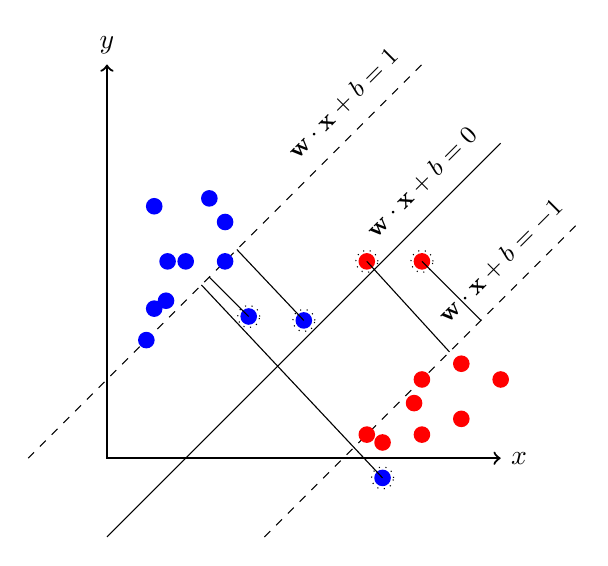
\begin{tikzpicture}[scale=1]
  % Draw axes
  \draw [<->,thick] (0,5) node (yaxis) [above] {$y$}
        |- (5,0) node (xaxis) [right] {$x$};
  % Draw line
  \draw (0,-1) -- (5,4); % y=x-1
  \draw[dashed] (-1,0) -- (4,5); % y=x+1
  \draw[dashed] (2,-1) -- (6,3); % y=x-3
  % \Draw labels
  \draw (4,3.5) node[rotate=45,font=\small] 
        {$\mathbf{w}\cdot \mathbf{x} + b = 0$};
  \draw (3,4.5) node[rotate=45,font=\small] 
        {$\mathbf{w}\cdot \mathbf{x} + b = 1$};
  \draw (5,2.5) node[rotate=45,font=\small] 
        {$\mathbf{w}\cdot \mathbf{x} + b = -1$};
  % \Draw distance
%  \draw[dotted] (4,5) -- (6,3);
%  \draw (5.25,4.25) node[rotate=-45] {$\frac{2}{\Vert \mathbf{w} \Vert}$};
%  \draw[dotted] (0,0) -- (0.5,-0.5);
%  \draw (0,-0.5) node[rotate=-45] {$\frac{b}{\Vert \mathbf{w} \Vert}$};
%  \draw[->] (2,1) -- (1.5,1.5);
%  \draw (1.85,1.35) node[rotate=-45] {$\mathbf{w}$};
  % \Draw negative dots
  \fill[blue] (0.5,1.5) circle (3pt);
  \fill[blue]   (1.5,2.5)   circle (3pt);
  \fill[blue] (1,2.5)     circle (3pt);
  \fill[blue] (0.75,2)    circle (3pt);
  \fill[blue] (0.6,1.9)   circle (3pt);
  \fill[blue] (0.77, 2.5) circle (3pt);
  \fill[blue] (1.5,3)     circle (3pt);
  \fill[blue] (1.3,3.3)   circle (3pt);
  \fill[blue] (0.6,3.2)   circle (3pt);
  \fill[blue] (1.8,1.8)     circle (3pt);
  \draw[dotted] (1.8,1.8) circle (4pt);
  \fill[blue] (2.5,1.75)     circle (3pt);
  \draw[dotted] (2.5,1.75) circle (4pt);
  \fill[blue] (3.5,-0.25)     circle (3pt);
  \draw[dotted] (3.5,-0.25) circle (4pt);
  \draw[-] (1.8,1.8) -- (1.3,2.3);
  \draw[-] (2.5,1.75) -- (1.65,2.65);
  \draw[-] (3.5,-0.25) -- (1.2,2.2);
  % \fill positive dots
  \fill[red] (4,1)     circle (3pt); 
  \fill[red] (3.3,.3)  circle (3pt); 
  \fill[red]     (4.5,1.2) circle (3pt); 
  \fill[red]     (4.5,.5)  circle (3pt); 
  \fill[red]     (3.9,.7)  circle (3pt); 
  \fill[red]     (5,1)     circle (3pt); 
  \fill[red]     (3.5,.2)  circle (3pt); 
  \fill[red]     (4,.3)    circle (3pt); 
  \fill[red]     (4,2.50)  circle (3pt);
  \draw[dotted]  (4,2.50)  circle (4pt);
  \fill[red]     (3.3,2.50)  circle (3pt);
  \draw[dotted]  (3.3,2.50)  circle (4pt);
  \draw[-,pin={[pin edge={->}]right:$\chi$}] (4,2.5) -- (4.75,1.75);
  \draw[-] (3.3,2.5) -- (4.35,1.35);
\end{tikzpicture}

    \end{figure}
\end{frame}
\begin{frame}
\frametitle{Introducing Slack Variables}
\begin{itemize}
  \item {\bf Separable Case}: To ensure zero training loss, constraint was
    \[
    y_n({\bf w}^\top {\bf x}_n + b) \ge 1\quad \forall{n = 1 \ldots N}
    \]
    \pause
  \item {\bf Non-separable Case}: Relax the constraint
    \begin{equation*}
      y_n({\bf w}^\top {\bf x}_n + b) \ge 1-\xi_n\quad \forall{n = 1 \ldots N}
    \end{equation*}
  \item $\xi_n$ is called \textcolor{blue}{\bf slack variable} ($\xi_n \ge 0$)
  \item \hilight{For misclassification, $\xi_n > 1$}
\end{itemize}
\end{frame}
\subsection{Optimization Constraints}
\begin{frame}
  \mode<presentation>
      {
        \frametitle{Relaxing the Constraint}
      }
      \begin{itemize}
      \item It is OK to have some misclassified training examples
          \begin{itemize}
          \item Some $\xi_n$'s will be non-zero
          \end{itemize}
          \pause
        \item Minimize the number of such examples
          \begin{itemize}
          \item Minimize $\hilightbox{\sum_{n=1}^N\xi_n}$
          \end{itemize}
        \item Optimization Problem for Non-Separable Case
      \end{itemize}
      \begin{empheq}[box=\widefbox]{equation*}
        \begin{aligned}
          & \underset{{\bf w},b}{\text{maximize}}
          & & f({\bf w},b) = \Vert{\bf w}\Vert^2 + C\sum_{n=1}^N\xi_n\\
          & \text{subject to}
          & & y_n({\bf w}^\top{\bf x}_n + b) \ge 1-\xi_n, \xi_n \ge 0\; n = 1, \ldots, N.
        \end{aligned}
      \end{empheq}
      \begin{itemize}
      \item $C$ controls the impact of margin and the margin error.
      \end{itemize}
\end{frame}
\begin{frame}
\mode<presentation>
    {
      \frametitle{Estimating Weights}
    }
    \begin{itemize}
    \item What is the role of $C$?
    \item Similar optimization procedure as for the separable case (QP for the dual)
    \item Weights have the same expression
      \[
        {\bf w} = \sum_{n=1}^N\alpha_ny_n{\bf x}_n
        \]
      \item All training examples exist in dot products ({\em kernelizable})
      \item Support vectors are slightly different
        \begin{enumerate}
        \item Points on the margin ($\xi_n = 0$)
        \item Inside the margin but on the correct side ($0 < \xi_n < 1$)
        \item On the wrong side of the hyperplane ($\xi_n \ge 1$)
        \end{enumerate}
    \end{itemize}
    \mode<article>
        {
          $C$ dictates if we focus more on maximizing the margin or reducing the training error.
        }
\end{frame}
\section{More About Kernels}
%\subsection{Motivation}
\begin{frame}
  \frametitle{Why Use Kernels?}
  \begin{columns}
    \begin{column}{0.4\textwidth}
      \begin{itemize}
      \item $x \in \Re$
      \item No linear separator
      \end{itemize}
      \begin{figure}
      \centering
      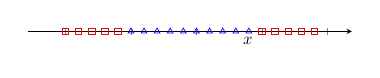
\begin{tikzpicture}[scale=0.6]
\begin{axis}[standard,xlabel=$x$,axis y line=none,xticklabels={,,},yticklabels={,,}]
\addplot [domain=-5:4, samples=10,mark=triangle,mark options={blue,solid},draw=none]{0};
\addplot+ [domain=-10:-6, samples=5,mark=square,mark options={red,solid},draw=none]{0};
\addplot+ [domain=5:9, samples=5,mark=square,mark options={red,solid},draw=none]{0};
\end{axis}
\end{tikzpicture}

    \end{figure}
  \end{column}
  \begin{column}{0.5\textwidth}
    \begin{itemize}
      \item Map $x \rightarrow \{x,x^2\}$
      \item Separable in 2D space
    \end{itemize}
    \begin{figure}
      \centering
    \begin{tikzpicture}[scale=0.6]
\begin{axis}[standard,xlabel=$x$,ylabel=$x^2$,xticklabels={,,},yticklabels={,,}]
\addplot [domain=-5:4, samples=10,mark=triangle,mark options={blue,solid},draw=none]{x+x^2};
\addplot+ [domain=-10:-6, samples=5,mark=square,mark options={red,solid},draw=none]{x+x^2};
\addplot+ [domain=5:9, samples=5,mark=square,mark options={red,solid},draw=none]{x+x^2};
\addplot+ [domain=-10:10, samples=5,mark=none,blue]{24};
\end{axis}
\end{tikzpicture}

  \end{figure}
  \end{column}
\end{columns}
\end{frame}
\begin{frame}
  \mode<presentation>
      {
        \frametitle{Another Example}
      }
      \begin{columns}
        \begin{column}{0.6\textwidth}
          \begin{itemize}
            \item ${\bf x} \in \Re^2$
            \item No linear separator
            \item Map ${\bf x} \rightarrow \{x_1^2,\sqrt{2}x_1x_2,x_2^2\}$
            \item A circle as the decision boundary
          \end{itemize}
        \end{column}
        \begin{column}{0.4\textwidth}
          \begin{figure}
            \centering
            \begin{tikzpicture}[scale=0.4]
\begin{axis}[]
\addplot[mark=triangle,mark options={blue}, draw=none] file {data0.txt};
\addplot+[mark=square,mark options={red},draw=none] file {data1.txt};
\only<2->{\draw[color=black] (axis cs:0,0) circle (240);}
\end{axis}
\end{tikzpicture}

            \begin{tikzpicture}[scale=0.4]
\begin{axis}[view={-175}{5}]
\addplot3[mark=triangle,mark options={blue}, draw=none] file {data4.txt};
\addplot3+[mark=square,mark options={red},draw=none] file {data5.txt};
\end{axis}
\end{tikzpicture}

          \end{figure}
        \end{column}
      \end{columns}
\end{frame}
\subsection{Gaussian Kernel}
\begin{frame}
  \mode<presentation>
      {
        \frametitle{The Gaussian Kernel}
      }
      \begin{itemize}
      \item The {\em squared dot product} kernel (${\bf x,x'} \in \Re^2$):
        \[
        k({\bf x},{\bf x}') = {\bf x}^\top{\bf x}' \triangleq {\bm \phi}({\bf x})^\top{\bm \phi}({\bf x}')
        \]
        \[
        {\bm \phi}({\bf x}) = \{x_1^2,\sqrt{2}x_1x_2,x_2^2\}
        \]
      \item What about the Gaussian kernel (radial basis function)?
        \begin{eqnarray*}
        k({\bf x},{\bf x}') & = & exp\left(-\frac{1}{2\sigma^2}||{\bf x}-{\bf x}'||^2\right)
        \end{eqnarray*}
      \end{itemize}
\end{frame}
\begin{frame}
  \mode<presentation>
      {
        \frametitle{Why is the Gaussian Kernel Mapping to Infinite Dimensions}
      }
      \begin{itemize}
        \item Assume $\sigma = 1$ and ${\bf x} \in \Re$ (denoted as $x$)
        \begin{eqnarray*}
          k(x,x') & = & exp(-x^2)exp(-x'^2)exp(2xx')\\
          & = & exp(-x^2)exp(-x'^2)\sum_{k=0}^\infty\frac{2^kx^kx'^k}{k!}\\
          & = & \sum_{k=0}^\infty\left(\frac{2^{k/2}}{\sqrt{k!}}x^kexp(-x^2)\right)\left(\frac{2^{k/2}}{\sqrt{k!}}x'^kexp(-x'^2)\right)
        \end{eqnarray*}
        \item {\em Using Maclaurin Series Expansion}
      \end{itemize}
      \begin{block}{}
      \[
      k(x,x') = 
      \begin{pmatrix}
        1\\
        2^{1/2}x^1 exp(-x^2)\\
        \frac{2^{2/2}}{2}x^2 exp(-x^2)\\
        \vdots\\
      \end{pmatrix}
      \times
      \begin{pmatrix}
        1\\
        2^{1/2}x'^1 exp(-x'^2)\\
        \frac{2^{2/2}}{2}x'^2 exp(-x'^2)\\
        \vdots\\
      \end{pmatrix}^\top
      \]
      \end{block}
\end{frame}
\mode<article>
    {
      One can note above that since computing the Gaussian kernel is same as taking a dot product of two vectors of infinite length, it is equivalent to mapping the input features into an infinite dimensional space.
    }
\begin{frame}
\frametitle{SVM Extensions}
\begin{enumerate}
  \item Multiple classes
    \begin{itemize}
      \item One vs.~Rest
      \item One vs.~One
    \end{itemize}
  \item One class SVM
  \item Transductive SVM (Semi-supervised Learning)
  \item Support Vector Regression
  \item Custom kernels (Use a {\em Gram} matrix)
\end{enumerate}
\end{frame}
\section*{References}
\label{sec:references}
\begin{frame}%[allowframebreaks]
  \mode<presentation>{
  \frametitle{References}}%
%  \bibliographystyle{abbrv}
%  \bibliography{../references}
\end{frame}
\end{document}
